\documentclass{beamer}
\usepackage[utf8]{inputenc}

\usepackage{utopia} %font utopia imported
\usepackage{multirow}

\usetheme{Madrid}
\usecolortheme{default}

\setbeamertemplate{footline}
{
  \leavevmode
  \hbox{
  \begin{beamercolorbox}[wd=1.01\paperwidth,ht=2.25ex,dp=1ex,right]{date in head/foot}
    \insertframenumber{} / \inserttotalframenumber\hspace*{2ex} 
  \end{beamercolorbox}}
  \vskip0pt%
}

%------------------------------------------------------------
%This block of code defines the information to appear in the
%Title page
\title{Classifying Human Driving Behavior via Deep Neural Networks}

\author{Jae Hoon Kim}

\institute{Drexel University}

\date{\today}

%End of title page configuration block
%------------------------------------------------------------



%------------------------------------------------------------
%The next block of commands puts the table of contents at the 
%beginning of each section and highlights the current section:

\AtBeginSection[]
{
  \begin{frame}
    \frametitle{Table of Contents}
    \tableofcontents[currentsection]
  \end{frame}
}
%------------------------------------------------------------


\begin{document}

%The next statement creates the title page.
\frame{\titlepage}


%---------------------------------------------------------
%This block of code is for the table of contents after
%the title page
\begin{frame}
\frametitle{Table of Contents}
\tableofcontents
\end{frame}
%---------------------------------------------------------

%%%%%%%%%%%%%%%%%%%%
%------------------%
%%%%%%%%%%%%%%%%%%%%
\section{Introduction}
\begin{frame}
\frametitle{Problem Statement}
\begin{itemize}
\item Modern car systems collect real-time data of the car status and driving behavior of the driver
\item Those data is worth for healthcare and research
\item Using driving behavior data to diagnose medical conditions
\end{itemize}
\end{frame}

\begin{frame}
\frametitle{Project Background}
\begin{itemize}
\item Classify driving simulation data from novice and expert drivers using several different neural network models
\item Explain LSTM and Auto-encoder
\item Compare result from three different neural network models
\end{itemize}
\end{frame}

%%%%%%%%%%%%%%%%%%%%
%------------------%
%%%%%%%%%%%%%%%%%%%%
\section{Background}
%%%%%%%%%%%%%%%%%%%%
\begin{frame}
\frametitle{Neural Networks - Introduction}
\begin{figure}[t!]
    \centering
    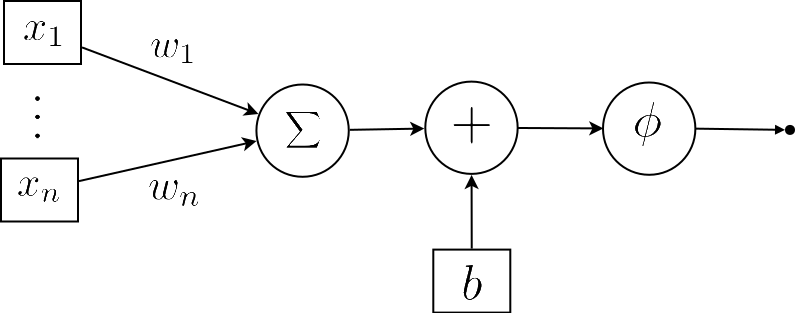
\includegraphics[width=0.5\textwidth]{../paper/pictures/figures/general_AN.png}
    \caption{General Artificial Neuron}
    \label{fig:general_AN}
\end{figure}

\begin{itemize}
\item An artificial neuron has input signals, weights, bias, and activation function
\end{itemize}
\end{frame}

%%%%%%%%%%%%%%%%%%%%
\begin{frame}
\frametitle{Neural Networks - Introduction}
\begin{columns}
\column{0.5\textwidth}
\begin{figure}[t!]
    \centering
    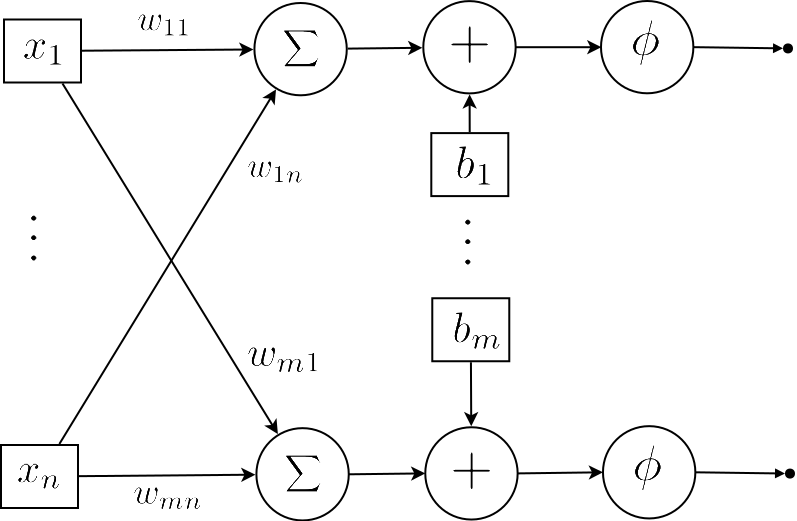
\includegraphics[width=\textwidth]{../paper/pictures/figures/detail_NN.png}
    \caption{Example of a Neural Network}
    \label{fig:detail_NN}
\end{figure}

\column{0.5\textwidth}
\begin{figure}[t!]
    \centering
    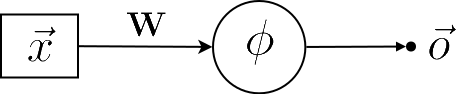
\includegraphics[width=0.6\textwidth]{../paper/pictures/figures/NN.png}
    \caption{Simplified Neural Network}
    \label{fig:NN}
\end{figure}
\end{columns}

\begin{itemize}
\item Neural network is a network made up many artificial neurons
\end{itemize}
\end{frame}

%%%%%%%%%%%%%%%%%%%%
\begin{frame}
\frametitle{Neural Networks - Forward Propagation}
\begin{figure}[t!]
    \centering
    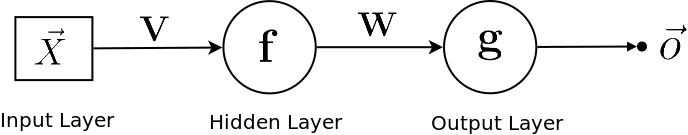
\includegraphics[width=0.45\textwidth]{../paper/pictures/figures/MLP.png}
    \caption{One Hidden Layer MLP}
    \label{fig:MLP}
\end{figure}

$$\vec{h} = \bold{f}(\vec{x}\bold{v}+\vec{c}) = \bold{f}(\vec{X}\bold{V})$$

$$\vec{o} = \bold{g}(\vec{h}\bold{w}+\vec{b}) = \bold{g}(\vec{H}\bold{W})$$

$$\vec{o} = \bold{g}(\bold{h}(\vec{x}\bold{v}+\vec{c})\bold{w}+\vec{b}) = \bold{g}(\bold{h}(\vec{X}\bold{V})\bold{W})$$
\end{frame}

%%%%%%%%%%%%%%%%%%%%
\begin{frame}
\frametitle{Neural Networks - Back Propagation}
\begin{figure}[t!]
    \centering
    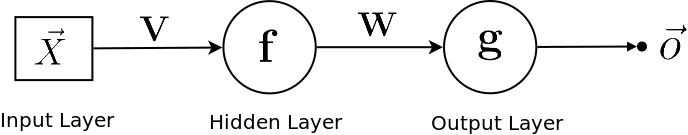
\includegraphics[width=0.45\textwidth]{../paper/pictures/figures/MLP.png}
    \caption{One Hidden Layer MLP}
    \label{fig:MLP}
\end{figure}

Activation Function:
$$f(z)=g(z)=sigm(z)=\frac{1}{1+e^{-z}}$$

Error Function:
$$J(\bold{V}, \bold{W}) = \frac{1}{2}\sum_{i}(y_i-o_i)^2 =\frac{1}{2}\sum_{i}(y_i-g(\bold{h}(\vec{X}\bold{V})\bold{W_i}))^2$$

\end{frame}

%%%%%%%%%%%%%%%%%%%%
\begin{frame}
\frametitle{Neural Networks - Back Propagation}
Update $W_{ij}$ - $i$th neuron for $j$th input:
\begin{figure}[t!]
    \centering
    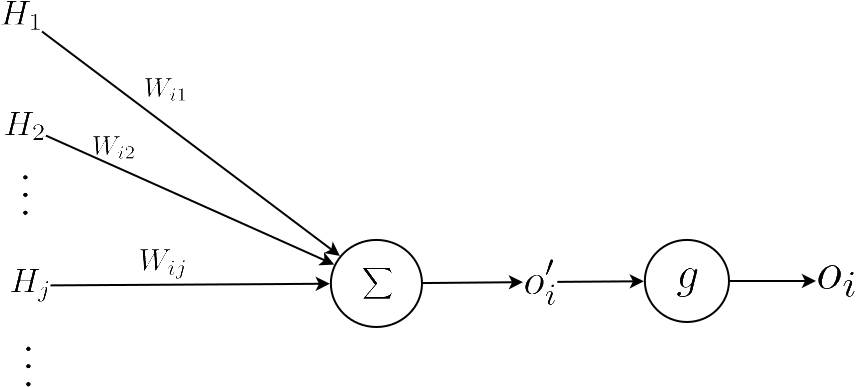
\includegraphics[width=0.5\textwidth]{../paper/pictures/figures/BP1.png}
    \caption{Back-propagation for $W_{ij}$}
    \label{fig:BP1}
\end{figure}

$$
{{W_{ij}}^{next}}
= W_{ij} - \eta\frac{\partial J}{\partial W_{ij}}
= W_{ij} - \eta\frac{\partial J}{\partial o_i}\frac{\partial o_i}{\partial o'_i}\frac{\partial o'_i}{\partial W_{ij}}
= W_{ij} + \eta(y_i-o_i)o_i(1-o_i)H_j
$$

Let
$$
\delta_i
= \frac{\partial J}{\partial o'_i}
= \frac{\partial J}{\partial o_i}\frac{\partial o_i}{\partial o'_i}
$$
\end{frame}

%%%%%%%%%%%%%%%%%%%%
\begin{frame}
\frametitle{Neural Networks - Back Propagation}
Update $V_{ij}$ - $i$th neuron for $j$th input:
\begin{figure}[t!]
    \centering
    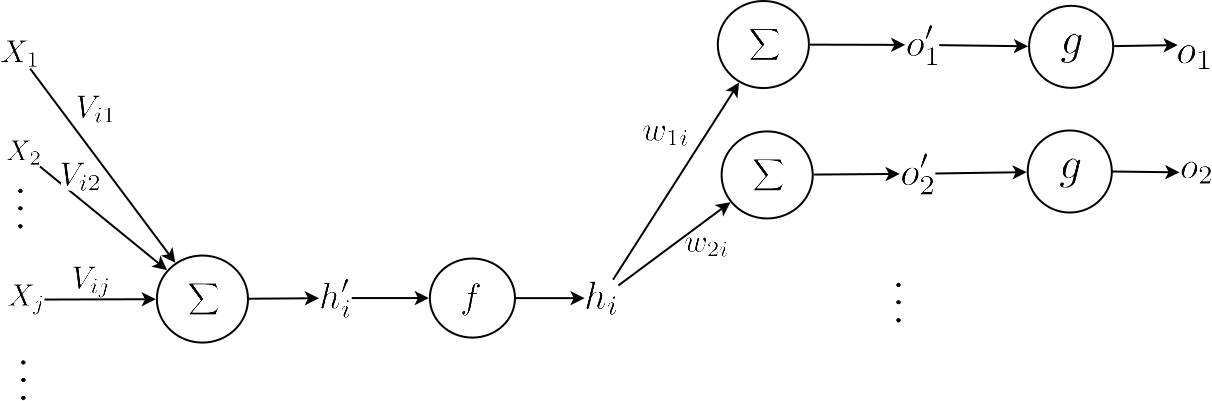
\includegraphics[width=0.9\textwidth]{../paper/pictures/figures/BP2.png}
    \caption{Back-propagation for $V_{ij}$}
    \label{fig:BP2}
\end{figure}
$$
{{V_{ij}}^{next}}
= V_{ij} - \eta\frac{\partial J}{\partial V_{ij}}
= V_{ij} - \eta\frac{\partial J}{\partial h_i}\frac{\partial h_i}{\partial h'_i}\frac{\partial h'_i}{\partial V_{ij}}
= V_{ij} - \eta\sum_k(\delta_kw_{ki})h_i(1-h_i)X_j
$$

\end{frame}

%%%%%%%%%%%%%%%%%%%%
\begin{frame}
\frametitle{Long Short Term Memory Networks (LSTM)}
\begin{columns}
\column{0.5\textwidth}
\begin{figure}[t!]
    \centering
    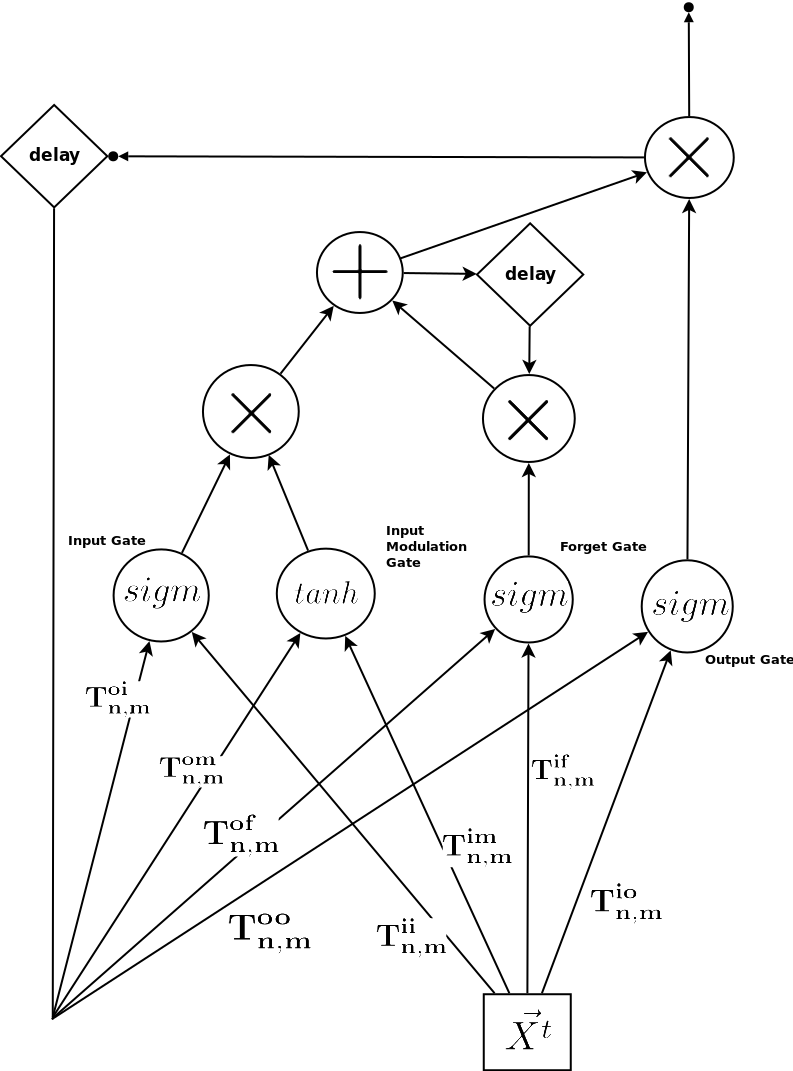
\includegraphics[width=0.8\textwidth]{../paper/pictures/figures/LSTM.png}
    \caption{LSTM}
    \label{fig:LSTM}
\end{figure}

\column{0.5\textwidth}
\begin{itemize}
\item Recurrent Neural Network
\item Four gates and Memory Cells handle long term dependencies
\end{itemize}
\end{columns}
\end{frame}

%%%%%%%%%%%%%%%%%%%%
\begin{frame}
\frametitle{Long Short Term Memory Networks (LSTM)}
Input gate:
$$\vec{i^t} = \bold{sigm}(\vec{X^t}\bold{T_{n,m}^{ii}} + \vec{H^{t-1}}\bold{T_{m,m}^{oi}})$$

Input modulation gate:
	$$\vec{m^t} = \bold{tanh}(\vec{X^t}\bold{T_{n,m}^{im}} + \vec{H^{t-1}}\bold{T_{m,m}^{om}})$$

Forget gate:
	$$\vec{f^t} = \bold{sigm}(\vec{X^t}\bold{T_{n,m}^{if}} + \vec{H^{t-1}}\bold{T_{m,m}^{of}})$$

Output gate:
	$$\vec{o^t} = \bold{sigm}(\vec{X^t}\bold{T_{n,m}^{io}} + \vec{H^{t-1}}\bold{T_{m,m}^{oo}})$$

Memory cells:
	$$\vec{c^t} = \vec{i^t} * \vec{m^t} + \vec{f^t} * \vec{c^{t-1}}$$

Result:
	$$\vec{h^t} = \vec{c^t} * \vec{o^t}$$
\end{frame}

%%%%%%%%%%%%%%%%%%%%
\begin{frame}
\frametitle{Auto-encoder (AE) - Single layer AE}
\begin{figure}[t!]
    \centering
    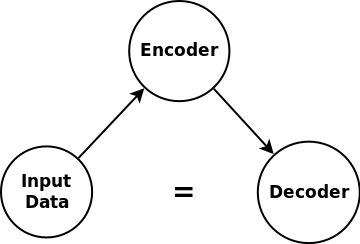
\includegraphics[width=0.35\textwidth]{../paper/pictures/figures/AE.png}
    \caption{Abstract structure of Auto-encoder}
    \label{fig:AE}
\end{figure}

Auto-encoder is a neural network to attempt to copy its inputs to its outputs
\end{frame}

%%%%%%%%%%%%%%%%%%%%
\begin{frame}
\frametitle{Auto-encoder (AE) - Single layer AE}
\begin{figure}[t!]
    \centering
    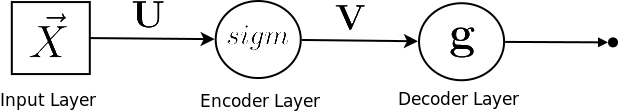
\includegraphics[width=0.4\textwidth]{../paper/pictures/figures/basic_AE.png}
    \caption{Basic Auto-encoder}
    \label{fig:basic_AE}
\end{figure}

$$\vec{e} = \bold{f}(\vec{X}\bold{U})$$

$$\vec{d} = \bold{g}(\vec{E}\bold{V})$$

$$E(\vec{x}, \vec{d}) = E(\vec{x}, \bold{g}(\vec{E}\bold{V})) = E(\vec{x}, \bold{g}(\bold{f}(\vec{x}\bold{u}+\vec{b_e})\bold{v}+\vec{b_d}))$$
\end{frame}

%%%%%%%%%%%%%%%%%%%%
\begin{frame}
\frametitle{Auto-encoder (AE) - Multiple layer AE}
\begin{figure}[t!]
    \centering
    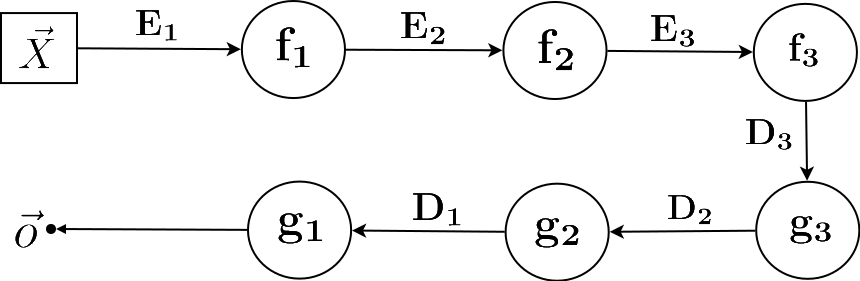
\includegraphics[width=0.6\textwidth]{../paper/pictures/figures/example_MAE.png}
    \caption{Multilayer Auto-encoder Example}
    \label{fig:example_MAE}
\end{figure}
\end{frame}

%%%%%%%%%%%%%%%%%%%%
\begin{frame}
\frametitle{Auto-encoder (AE) - Multiple layer AE}
\begin{figure}[t!]
    \centering
    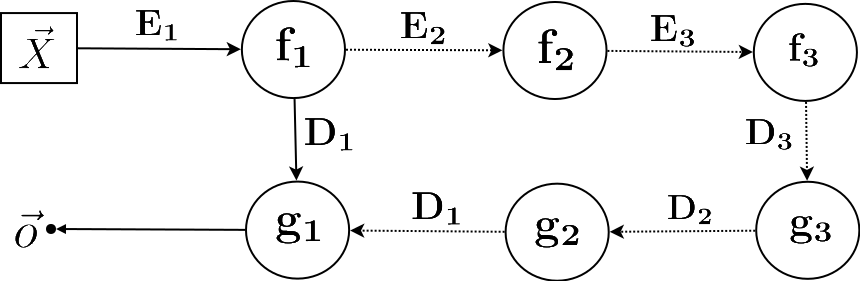
\includegraphics[width=0.25\textwidth]{../paper/pictures/figures/train_MAE1.png}
    \caption{Pretraining First Step}
    \label{fig:train_MAE1}
\end{figure}

$$E(input, data\_from\_first\_decoder)$$
$$=E(\vec{x}, \bold{g_1}(\bold{f_1}(\vec{X}\bold{E_1})\bold{D_1}))$$
\end{frame}

%%%%%%%%%%%%%%%%%%%%
\begin{frame}
\frametitle{Auto-encoder (AE) - Multiple layer AE}
\begin{figure}[t!]
    \centering
    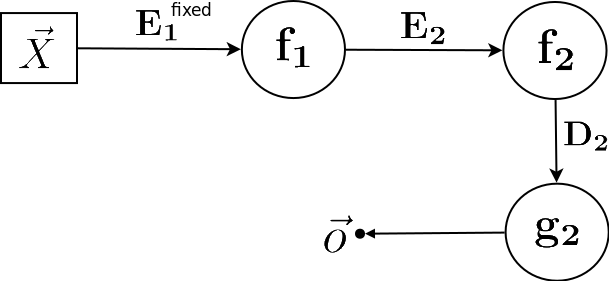
\includegraphics[width=0.4\textwidth]{../paper/pictures/figures/train_MAE2.png}
    \caption{Pretraining Second Step}
    \label{fig:train_MAE2}
\end{figure}

$$E(data\_from\_first\_encoder, data\_from\_second\_decoder)$$
$$=E(\bold{f_1}(\vec{X}\bold{E_1^{fixed}}), \bold{g_2}(\bold{f_2}(\bold{f_1}(\vec{X}\bold{E_1^{fixed}})\bold{E_2})\bold{D_2}))$$
\end{frame}

%%%%%%%%%%%%%%%%%%%%
\begin{frame}
\frametitle{Auto-encoder (AE) - Multiple layer AE}
\begin{figure}[t!]
    \centering
    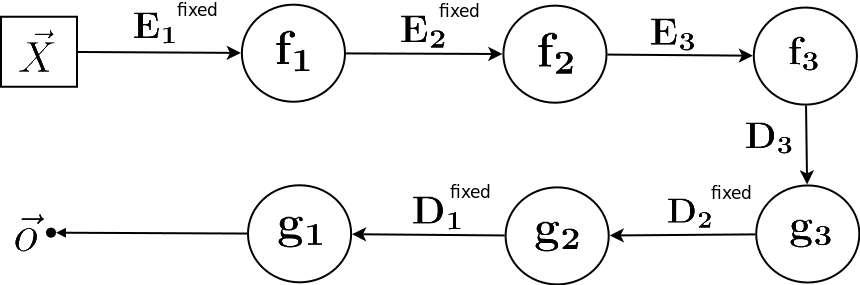
\includegraphics[width=0.6\textwidth]{../paper/pictures/figures/train_MAE3.png}
    \caption{Pretraining Thrid Step}
    \label{fig:train_MAE3}
\end{figure}

$$E(data\_from\_second\_encoder, data\_from\_third\_decoder)$$
$$=E(\bold{f_2}(\bold{f_1}(\vec{X}\bold{E_1^{fixed}})\bold{E_2^{fixed}}), \bold{g_3}(\bold{f_3}(\bold{f_2}(\bold{f_1}(\vec{X}\bold{E_1^{fixed}})\bold{E_2^{fixed}})\bold{E_3})\bold{D_3}))$$
\end{frame}

%%%%%%%%%%%%%%%%%%%%
\begin{frame}
\frametitle{Auto-encoder (AE) - Multiple layer AE}
\begin{figure}[t!]
    \centering
    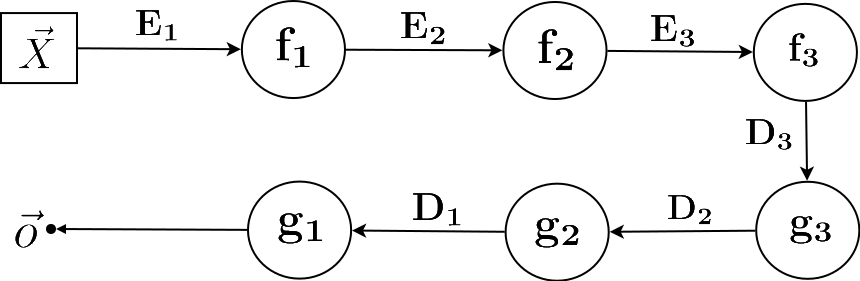
\includegraphics[width=0.6\textwidth]{../paper/pictures/figures/example_MAE.png}
    \caption{Multilayer Auto-encoder Example}
    \label{fig:example_MAE}
\end{figure}

$$E(input, output)$$
$$=E(\vec{x}, \bold{g_1}(\bold{g_2}(\bold{g_3}(\bold{f_3}(\bold{f_2}(\bold{f_1}(\vec{X}\bold{E_1})\bold{E_2})\bold{E_3})\bold{D_3})\bold{D_2})\bold{D_1}))$$
\end{frame}


%%%%%%%%%%%%%%%%%%%%
%------------------%
%%%%%%%%%%%%%%%%%%%%
\section{Data Set}
%%%%%%%%%%%%%%%%%%%%
\begin{frame}
\frametitle{Data Set}
\begin{itemize}
\item Collected in the high-fidelity simulator of the Center for Injury Research Prevention Studies at the \textit{Children's Hospital of Philadelphia} (CHOP)
\item 16 traces = 4 tracks $\times$ (2 expert drivers + 2 inexpert drivers)
\item 100 features collected at 60Hz
	\begin{itemize}
	\item Car status: velocity, steer, Brake, throttle and etc.
	\item Environment status: current speed limit, and etc.
	\item instruction: left turn, right turn, and etc.
	\end{itemize}
\item Two datasets
	\begin{itemize}
	\item {\em raw dataset}: 98 features without time stamps
	\item {\em filtered dataset}: 23 features - more important features from 100 features
	\end{itemize}
\end{itemize}

\end{frame}

%%%%%%%%%%%%%%%%%%%%
\begin{frame}
\frametitle{Data Set}
\begin{columns}
\column{0.5\textwidth}
\begin{table}[tb]
\centering
\caption{Length of each of the traces}
\label{tbl:traces}
\resizebox{0.8\textwidth}{!}{\begin{tabular}{|l|l|l|l|}
\hline
{\em Trace}   & {\em Driver}    & {\em Track}  & {\em Length} \\ \hline
Trace0  & Expert0   & Track0 & 50029  \\
Trace1  & Expert0   & Track1 & 26375  \\
Trace2  & Expert0   & Track2 & 29629  \\
Trace3  & Expert0   & Track3 & 26298  \\
Trace4  & Expert1   & Track0 & 51295  \\
Trace5  & Expert1   & Track1 & 26674  \\
Trace6  & Expert1   & Track2 & 29680  \\
Trace7  & Expert1   & Track3 & 27075  \\
Trace8  & Inexpert0 & Track0 & 49691  \\
Trace9  & Inexpert0 & Track1 & 30058  \\
Trace10 & Inexpert0 & Track2 & 26441  \\
Trace11 & Inexpert0 & Track3 & 27373  \\
Trace12 & Inexpert1 & Track0 & 47658  \\
Trace13 & Inexpert1 & Track1 & 29380  \\
Trace14 & Inexpert1 & Track2 & 26684  \\
Trace15 & Inexpert1 & Track3 & 27255  \\ \hline
\end{tabular}}
\end{table}

\column{0.5\textwidth}
\begin{itemize}
\item Min: 26298

(about 7 minutes 18 seconds)
\item Max: 51295 

(about 14 minutes 15 seconds)
\item Average: 33224.6875

(about 9 minutes 13 seconds)
\end{itemize}
\end{columns}
\end{frame}

%%%%%%%%%%%%%%%%%%%%
%------------------%
%%%%%%%%%%%%%%%%%%%%
\section{Technical Approach}
%%%%%%%%%%%%%%%%%%%%
\begin{frame}
\frametitle{Cross Validation $\&$ Normalization}
\begin{columns}
\column{0.5\textwidth}
\begin{figure}[tb]
    \centering
    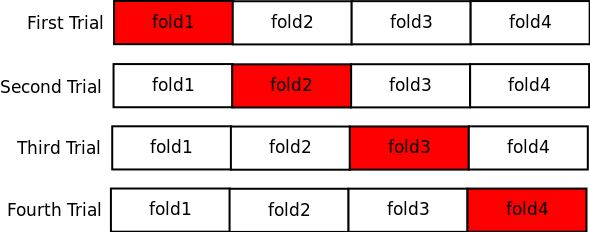
\includegraphics[width=\textwidth]{../paper/pictures/figures/CV.png}
    \caption{4 Folds Cross Validation}
    \label{fig:CV}
\end{figure}

\column{0.5\textwidth}
\begin{itemize}
\item Cross Validation
	\begin{itemize}
	\item To validate experiment models when data is not large enough
	\item Divides a data set into $K$ folds
	\item Uses the $i$th fold as the test set and other folds as the training set
	\end{itemize}
\item Normalization
	\begin{itemize}
	\item Normalize training set
	
	(mean 0, std 1)
	\item Normalize test set by mean and standard deviation of training set
	\end{itemize}
\end{itemize}
\end{columns}
\end{frame}

%%%%%%%%%%%%%%%%%%%%
\begin{frame}
\frametitle{First Model}
\begin{figure}[t!]
    \centering
    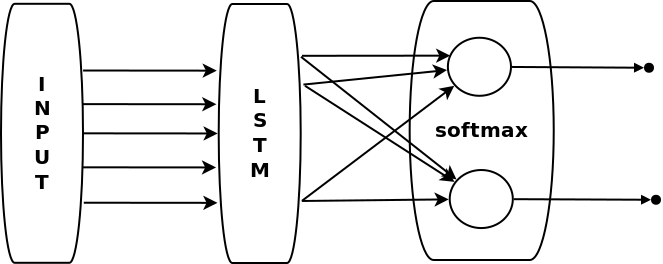
\includegraphics[width=0.6\textwidth]{../paper/pictures/figures/exp_NN1.png}
    \caption{First experiment NN}
    \label{fig:exp_NN1}
\end{figure}

\begin{itemize}
\item Hidden neurons in LSTM: 16, 32, 64, 128, and 256
\item Without Auto-encoder on {\em filtered dataset}
\end{itemize}
\end{frame}

%%%%%%%%%%%%%%%%%%%%
\begin{frame}
\frametitle{Second Model}
\begin{figure}[t!]
    \centering
    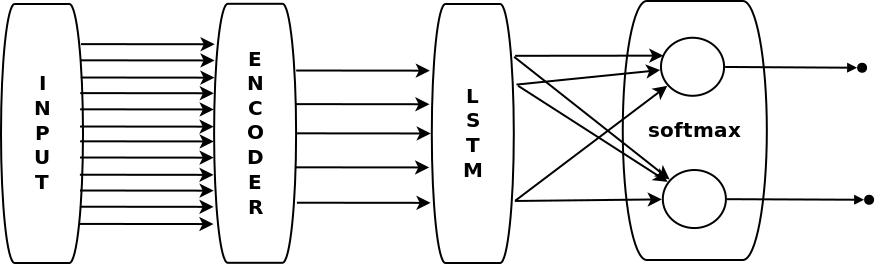
\includegraphics[width=0.7\textwidth]{../paper/pictures/figures/exp_NN2.png}
    \caption{Second experiment NN}
    \label{fig:exp_NN2}
\end{figure}

\begin{itemize}
\item Hidden neurons in LSTM: 16, 32, 64, 128, and 256
\item With Single layer Auto-encoder on {\em raw dataset}:

98 features $\rightarrow$ 25 features
\end{itemize}
\end{frame}

%%%%%%%%%%%%%%%%%%%%
\begin{frame}
\frametitle{Third Model}
\begin{figure}[t!]
    \centering
    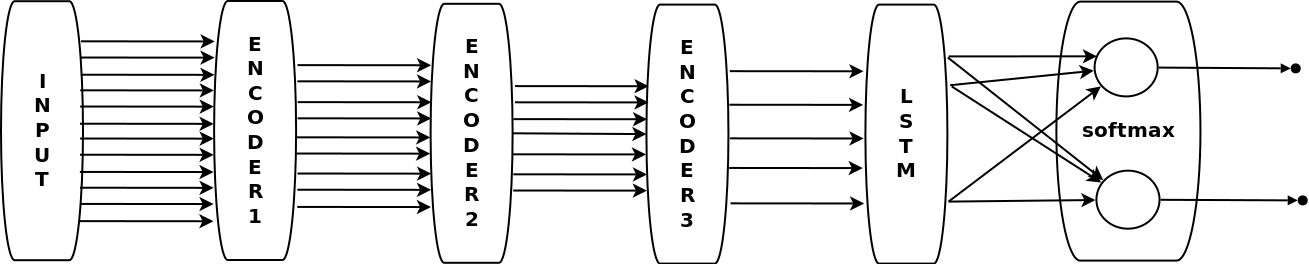
\includegraphics[width=0.9\textwidth]{../paper/pictures/figures/exp_NN3.png}
    \caption{Third experiment NN}
    \label{fig:exp_NN3}
\end{figure}

\begin{itemize}
\item Hidden neurons in LSTM: 16, 32, 64, 128, and 256
\item With Three layer Auto-encoder on {\em raw dataset}:

98 features $\rightarrow$ 75 features $\rightarrow$ 50 features $\rightarrow$ 25 features
\end{itemize}
\end{frame}

%%%%%%%%%%%%%%%%%%%%
\begin{frame}
\frametitle{Sampling}
\begin{columns}
\column{0.5\textwidth}
\begin{itemize}
\item Period
	\begin{itemize}
	\item 1 over 10
	\item 1 over 20
	\item 1 over 50
	\end{itemize}
\item Sampling Methods
	\begin{itemize}
	\item Last sample from each period
	\item Mean of each period
	\item Gaussian filtered value of each period
	\end{itemize}
\end{itemize}

\column{0.5\textwidth}
\begin{table}[]
\centering
\caption{Sampling and Models}
\label{sampling_models}
\resizebox{0.8\textwidth}{!}{\begin{tabular}{|c|c|c|}
\hline
Period                     & Method   & Model                         \\ \hline
\multirow{3}{*}{1 over 10} & last     & \textit{first, second, third} \\ \cline{2-3} 
                           & mean     & \textit{first}                \\ \cline{2-3} 
                           & gaussian & \textit{first}                \\ \hline
\multirow{3}{*}{1 over 20} & last     & \textit{first}                \\ \cline{2-3} 
                           & mean     & \textit{first}                \\ \cline{2-3} 
                           & gaussian & \textit{first}                \\ \hline
\multirow{3}{*}{1 over 50} & last     & \textit{first}                \\ \cline{2-3} 
                           & mean     & \textit{first}                \\ \cline{2-3} 
                           & gaussian & \textit{first}                \\ \hline
\end{tabular}}
\end{table}
\end{columns}
\end{frame}

%%%%%%%%%%%%%%%%%%%%
%\begin{frame}
%\frametitle{Environment}
%Tux
%\begin{itemize}
%\item Processors:
%\item Memory:
%\item Tensorflow 0.12.1
%\end{itemize}
%\end{frame}

%%%%%%%%%%%%%%%%%%%%
%------------------%
%%%%%%%%%%%%%%%%%%%%
\section{Experimental Result}

%%%%%%%%%%%%%%%%%%%%
\begin{frame}
\frametitle{First Model with 1 over 50}
\begin{columns}
\column{0.5\textwidth}
\begin{figure}[tb]
    \centering
    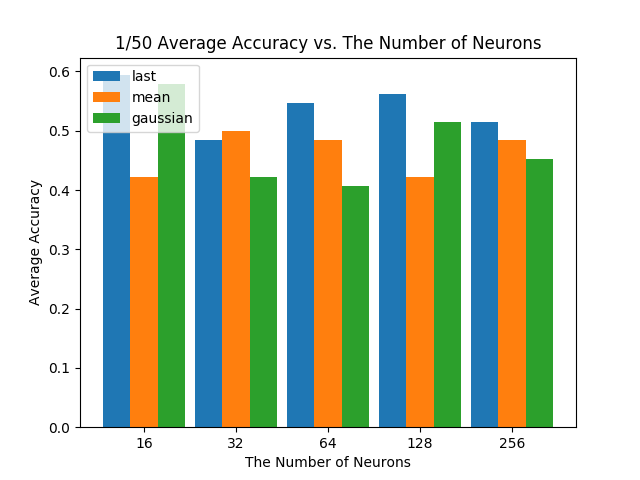
\includegraphics[width=\textwidth]{../paper/pictures/result_pictures/filtered_1_50_result.png}
    \caption{Result of first model with 1 over 50 {\em filtered dataset}}
    \label{fig:filter_1_50}
\end{figure}

\column{0.5\textwidth}
\begin{itemize}
\item Best: 0.59375 (59.375\%) on {\em last} and 16 neurons
\item Worst: 0.40625 (40.625\%) on {\em gaussian} and 64 neurons
\item Average: 0.492708 (49.2708\%)
\end{itemize}
\end{columns}
\end{frame}

%%%%%%%%%%%%%%%%%%%%
\begin{frame}
\frametitle{First Model with 1 over 20}
\begin{columns}
\column{0.5\textwidth}
\begin{figure}[t!]
    \centering
    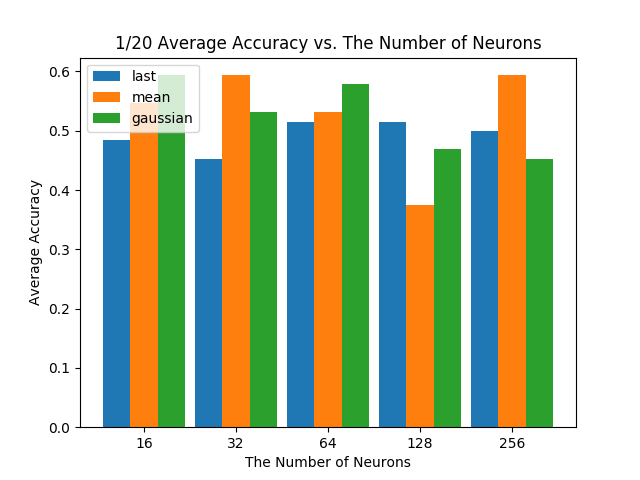
\includegraphics[width=\textwidth]{../paper/pictures/result_pictures/filtered_1_20_result.png}
    \caption{Result of first model with 1 over 20 {\em filtered dataset}}
    \label{fig:filter_1_20}
\end{figure}

\column{0.5\textwidth}
\begin{itemize}
\item Best: 0.59375 (59.375\%) on {\em mean} and 32 and 256 neurons
\item Worst: 0.375 (37.5\%) on {\em mean} and 128 neurons
\item Average: 0.515625 (51.5625\%)
\end{itemize}
\end{columns}
\end{frame}

%%%%%%%%%%%%%%%%%%%%
\begin{frame}
\frametitle{First Model with 1 over 10}
\begin{columns}
\column{0.5\textwidth}
\begin{figure}[t!]
    \centering
    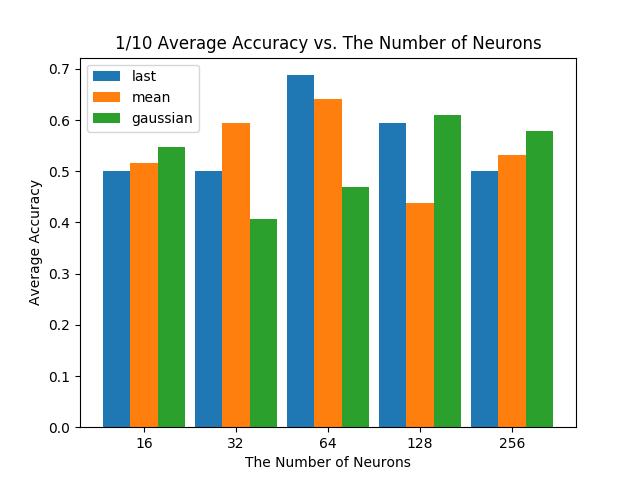
\includegraphics[width=\textwidth]{../paper/pictures/result_pictures/filtered_1_10_result.png}
    \caption{Result of first model with 1 over 10 {\em filtered dataset}}
    \label{fig:filter_1_10}
\end{figure}

\column{0.5\textwidth}
\begin{itemize}
\item Best: 0.6875 (68.75\%) on {\em last} and 64 neurons
\item Worst: 0.40625 (40.625\%) on {\em gaussian} and 32 neurons
\item Average: 0.540625 (54.00625\%)
\end{itemize}
\end{columns}
\end{frame}

%%%%%%%%%%%%%%%%%%%%
\begin{frame}
\frametitle{Comparison of three models with 1 over 10, {\em last} method}
\begin{columns}
\column{0.5\textwidth}
\begin{figure}[t!]
    \centering
    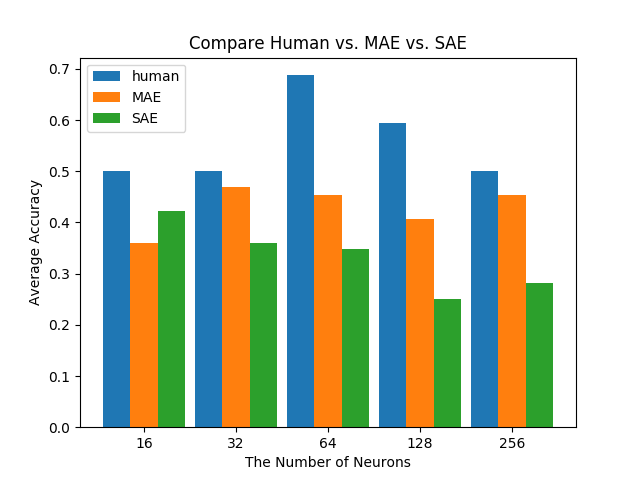
\includegraphics[width=\textwidth]{../paper/pictures/result_pictures/compare_result_last_1_10.png}
    \caption{Result of three models with 1 over 10, {\em last} method}
    \label{fig:compare_result_last_1_10}
\end{figure}

\column{0.5\textwidth}
Models with Auto-encoder show worse performance
\end{columns}
\end{frame}

%%%%%%%%%%%%%%%%%%%%
\begin{frame}
\frametitle{Comparison of three models with 1 over 10, {\em last} method}
\begin{figure}[t!]
    \centering
    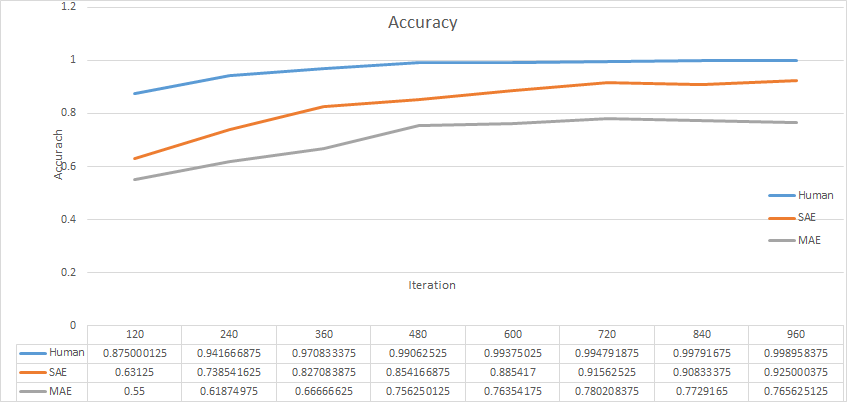
\includegraphics[width=\textwidth]{../paper/pictures/result_pictures/three_models_comparison_accuracy.png}
    \caption{Three Models Training Accuracy}
    \label{fig:three_models_comparison_accuracy}
\end{figure}
\end{frame}

%%%%%%%%%%%%%%%%%%%%
\begin{frame}
\frametitle{Comparison of three models with 1 over 10, {\em last} method}
\begin{figure}[t!]
    \centering
    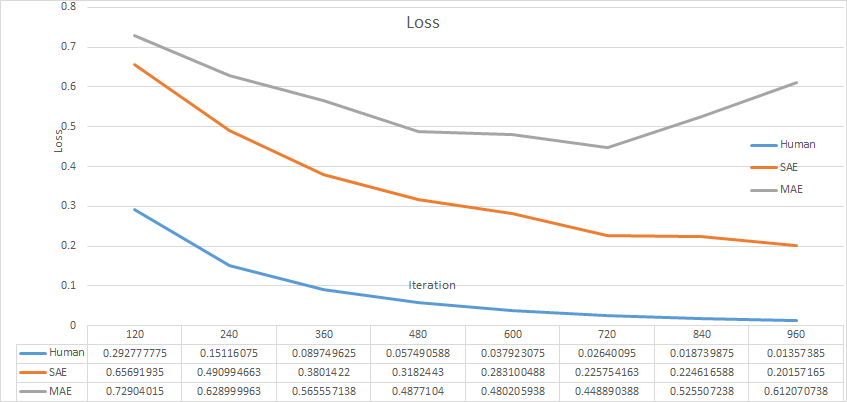
\includegraphics[width=\textwidth]{../paper/pictures/result_pictures/three_models_comparison_loss.png}
    \caption{Three Models Training Loss}
    \label{fig:three_models_comparison_loss}
\end{figure}
\end{frame}

%%%%%%%%%%%%%%%%%%%%
\begin{frame}
\frametitle{Problems with second and third models}
\begin{figure}[t!]
    \centering
    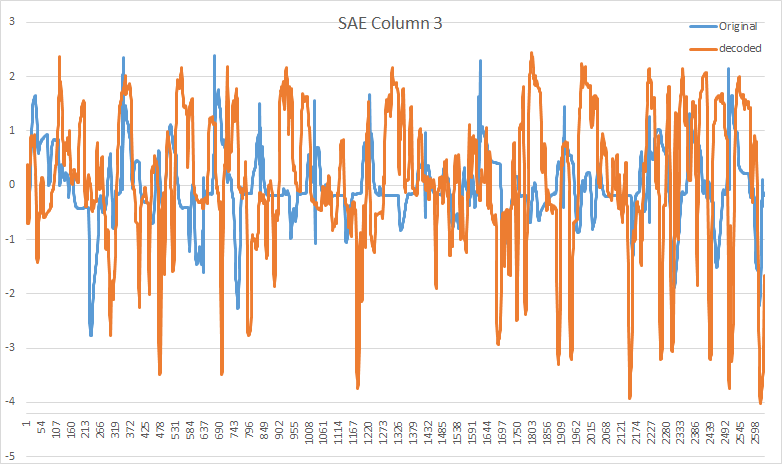
\includegraphics[width=\textwidth]{../paper/pictures/result_pictures/SAE_Column_3.png}
    \caption{SAE, AE Error for Column 3}
    \label{fig:sae_error_c3}
\end{figure}
\end{frame}

%%%%%%%%%%%%%%%%%%%%
\begin{frame}
\frametitle{Problems with second and third models}
\begin{figure}[t!]
    \centering
    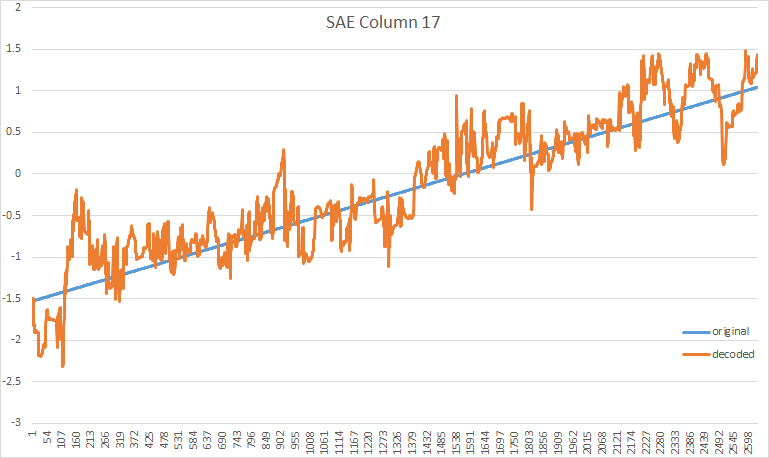
\includegraphics[width=\textwidth]{../paper/pictures/result_pictures/SAE_Column_17.png}
    \caption{SAE, AE Error for Column 17}
    \label{fig:sae_error_c17}
\end{figure}
\end{frame}

%%%%%%%%%%%%%%%%%%%%
\begin{frame}
\frametitle{Problems with second and third models}
\begin{figure}[t!]
    \centering
    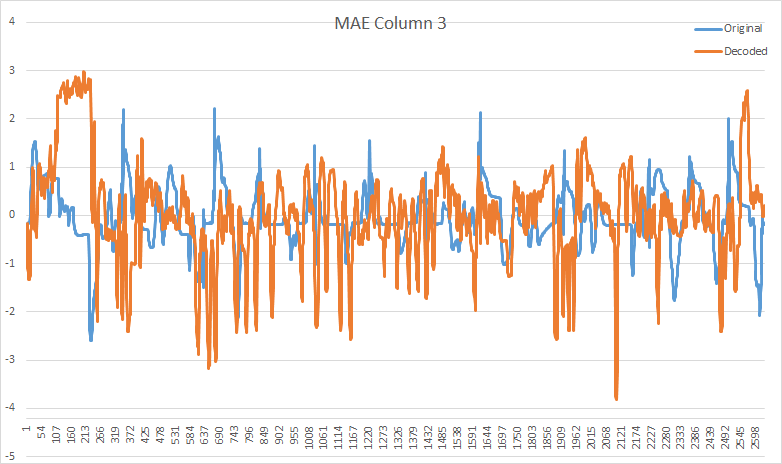
\includegraphics[width=\textwidth]{../paper/pictures/result_pictures/MAE_Column_3.png}
    \caption{MAE, AE Error for Column 3}
    \label{fig:mae_error_c3}
\end{figure}
\end{frame}

%%%%%%%%%%%%%%%%%%%%
\begin{frame}
\frametitle{Problems with second and third models}
\begin{figure}[t!]
    \centering
    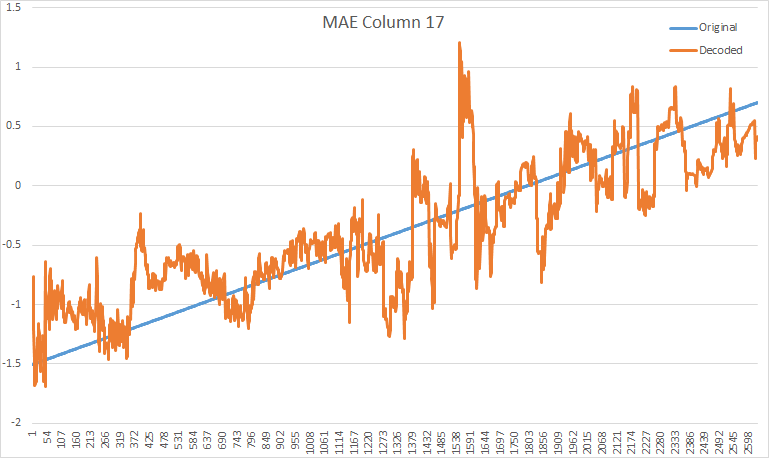
\includegraphics[width=\textwidth]{../paper/pictures/result_pictures/MAE_Column_17.png}
    \caption{MAE, AE Error for Column 17}
    \label{fig:mae_error_c17}
\end{figure}
\end{frame}

%%%%%%%%%%%%%%%%%%%%
%------------------%
%%%%%%%%%%%%%%%%%%%%
\section{Conclusion}
%%%%%%%%%%%%%%%%%%%%
\begin{frame}
\frametitle{Conclusion - Data Size}
\begin{itemize}
\item The number of samples in trace

From result of experiment with different re-sampled periods, more densely re-sampled data gives better performance

\item The number of traces

12 traces are not enough to train proposed neural networks

\end{itemize}
\end{frame}

%%%%%%%%%%%%%%%%%%%%
\begin{frame}
\frametitle{Conclusion - Limitation of Auto-encoders}
\begin{itemize}
\item No optimize transfer matrices

When Auto-encoder tries to reduce dimensions, if encoder and decoder transfer matrices are not exist, encoded data has noise. It can make hard to train following neural networks.

\item Always try to keep all information

Auto-encoder does not ignore or exclude unimportant features

\end{itemize}
\end{frame}

%%%%%%%%%%%%%%%%%%%%
\begin{frame}
\frametitle{Conclusion - Problem in training MAE}
\begin{itemize}
\item Training time

Processing of pretraining takes long time

\item Learn error from previous layer during pretraining

Fix previous layer while follow auto-encoder layer is trained

\end{itemize}

\begin{figure}[t!]
    \centering
    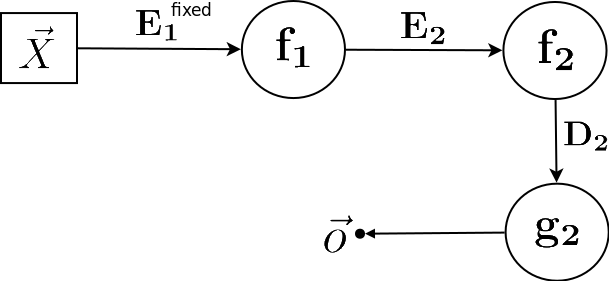
\includegraphics[width=0.4\textwidth]{../paper/pictures/figures/train_MAE2.png}
    \caption{Pretraining Second Step}
    \label{fig:train_MAE2}
\end{figure}
\end{frame}

%%%%%%%%%%%%%%%%%%%%
%------------------%
%%%%%%%%%%%%%%%%%%%%
\section{Future Work}
%%%%%%%%%%%%%%%%%%%%
\begin{frame}
\frametitle{Future Work}
\begin{itemize}
\item Experiment with more traces
\item Research auto-encoder that accept some form of supervision and reduce dimensions with the ability to ignore unimportant features and keep information from the important features
\item Try different way to train MAE
\end{itemize}
\end{frame}

%%%%%%%%%%%%%%%%%%%%
\begin{frame}
\frametitle{Future Work}
\begin{figure}[t!]
    \centering
    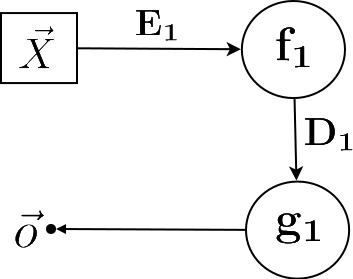
\includegraphics[width=0.25\textwidth]{../paper/pictures/figures/train_new_MAE1.png}
    \caption{First Step of New Way to train MAE}
    \label{fig:train_NMAE1}
\end{figure}

$$E(input, output)$$
$$=E(\vec{x}, \bold{g_1}(\bold{f_1}(\vec{X}\bold{E_1})\bold{D_1}))$$
\end{frame}

%%%%%%%%%%%%%%%%%%%%
\begin{frame}
\frametitle{Future Work}
\begin{figure}[t!]
    \centering
    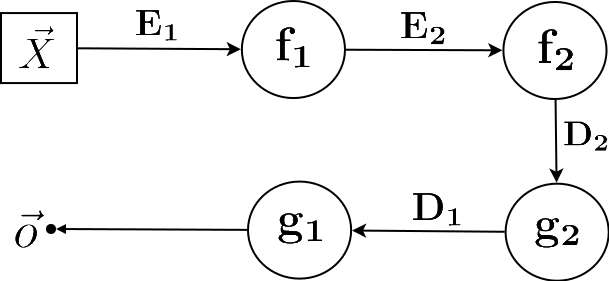
\includegraphics[width=0.4\textwidth]{../paper/pictures/figures/train_new_MAE2.png}
    \caption{Second Step of New Way to train MAE}
    \label{fig:train_NMAE2}
\end{figure}

$$E(input, output)$$
$$=E(\vec{x}, \bold{g_1}(\bold{g_2}(\bold{f_2}(\bold{f_1}(\vec{X}\bold{E_1})\bold{E_2})\bold{D_2})\bold{D_1}))$$
\end{frame}

%%%%%%%%%%%%%%%%%%%%
\begin{frame}
\frametitle{Future Work}
\begin{figure}[t!]
    \centering
    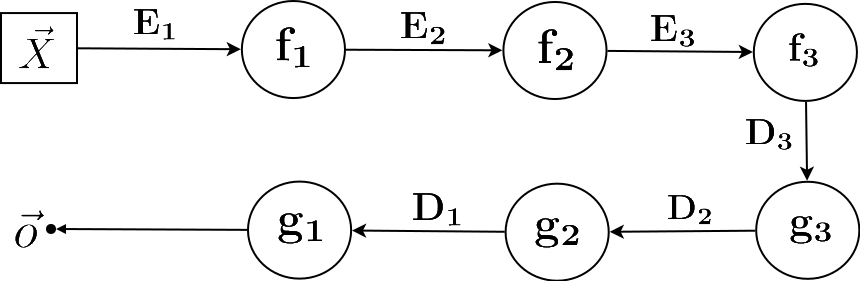
\includegraphics[width=0.6\textwidth]{../paper/pictures/figures/train_new_MAE3.png}
    \caption{Thrid Step of New Way to train MAE}
    \label{fig:train_NMAE3}
\end{figure}

$$E(input, output)$$
$$=E(\vec{x}, \bold{g_1}(\bold{g_2}(\bold{g_3}(\bold{f_3}(\bold{f_2}(\bold{f_1}(\vec{X}\bold{E_1})\bold{E_2})\bold{E_3})\bold{D_3})\bold{D_2})\bold{D_1}))$$
\end{frame}

%%%%%%%%%%%%%%%%%%%%
%------------------%
%%%%%%%%%%%%%%%%%%%%
\begin{frame}
\begin{center} 
\Huge Thank You 
\end{center} 
\end{frame}


%\begin{frame}[allowframebreaks]
%\frametitle{References}
%\bibliographystyle{amsalpha}
%\bibliography{../paper/references.bib}
%\end{frame}

\end{document}
